DOM

\section{Wizualizacja}
\label{sec:wizualizacja}

Poniższa sekcja zawiera próbę analizy dostępnych metod prezentacji danych zarówno zbiorów punktów, zdjęć i animacji. Główną uwagę zwrócono na 3 główne sposoby wizualizacji grafik. Ostatnia część zawiera zbiór dostępnych funkcjonalności, stanowi przewodnik po dostępnych możliwościach i ukazuje w jaki sposób można personalizować dane.


\subsection{Rodzaje map}
\label{sec:Rodzaje map}

Tworząc aplikację która ma dostarczać informacji korzystających z map należy zapoznać się dostępnymi źródłami. Z powodu szrokiego wyboru poniżej omówione zostaną jedynie aplikacje które dostarczają informacji ogólnoświatowych. Na polskim rynku dostępnych jest kilka rozwiązań, ich główną wadą jest ograniczenie do terytorium Polski, dodatkowo często nie dostarczają one obrazów satelitarnych, są to m.in. \underline{\texttt{http://zumi.pl}}


\subsubsection{Google Maps}
\label{subsec:Google Maps}
\nocite{googlemapsbegin}
Rysunek \ref{fig:googleMaps_1} przedstawia obraz otrzymany w aplikacji Google Maps. Dodatkowo włączona opcja prezentacji natężenia ruchu jedynie potwierdza duże możliwości i łatwość obsługi. Przyjazny interfejs sprawia że praca jest prosta i pozwala na osiągnięcie bardzo dobrych wyników.


\begin{figure}[H]
  \centering
    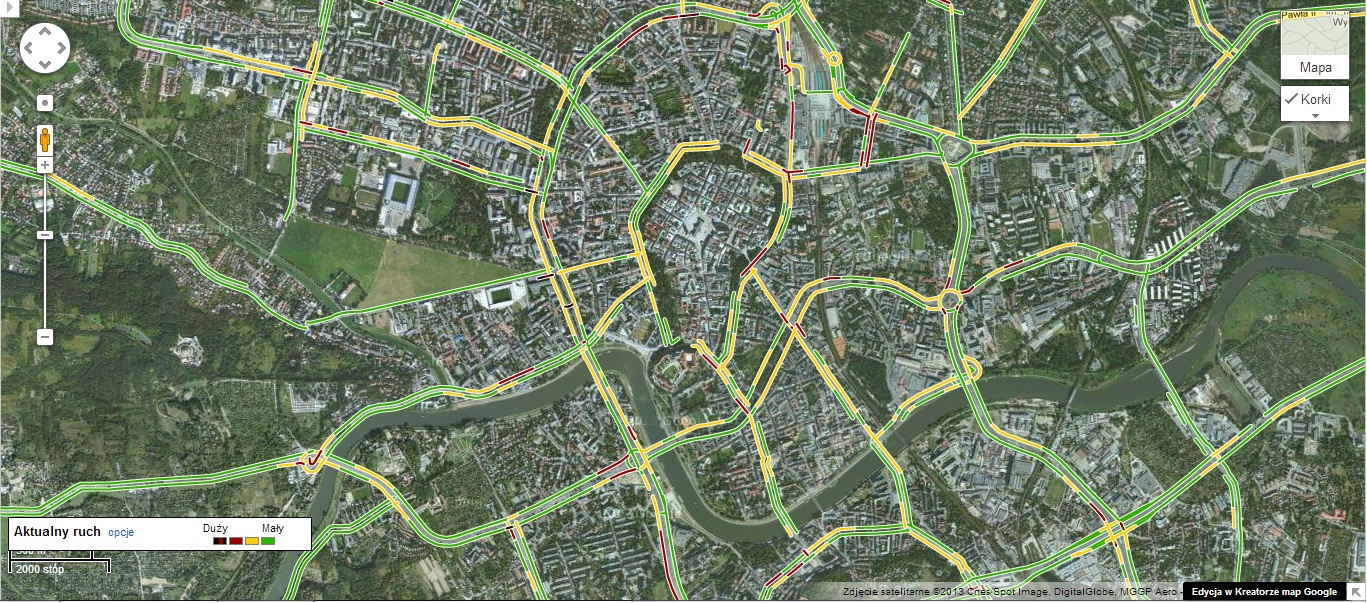
\includegraphics[width=100mm]{ge/gm_1.jpg}
  \caption{Google Maps.}
  \label{fig:googleMaps_1}
\end{figure}


\subsubsection{Windows Maps}
\label{subsec:Windows Maps}

Rysunek \ref{fig:bingMaps_1} przedstawia obraz otrzymany wykorzystując Bing Maps. W tym konkretnym przykładzie widzimy znaczną różnicę kolorów, obecność chmur pomniejsza wartość tych zdjęć. Należy wspomnieć o znacznie uboższym interfejsie dostarczanym użytkownikowi, interakcja jest w znacznym stopniu uboższa.

\begin{figure}[H]
  \centering
    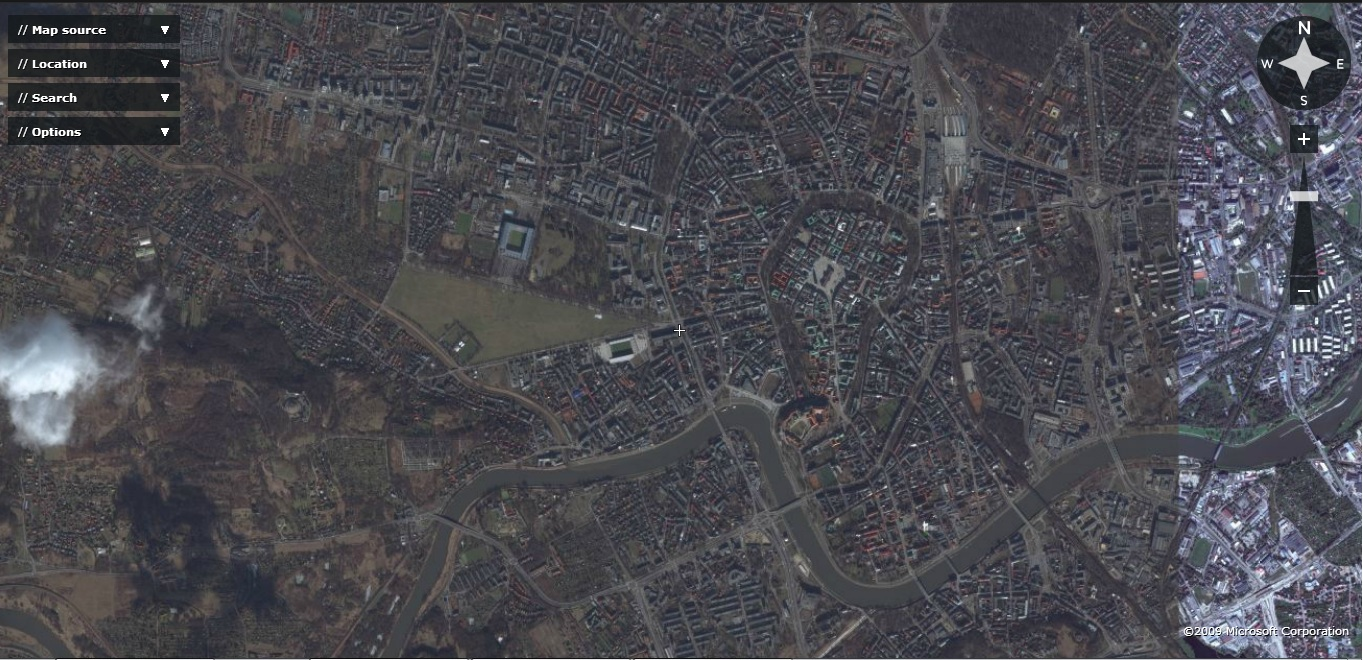
\includegraphics[width=100mm]{ge/bing_1.jpg}
  \caption{Bing Maps.}
  \label{fig:bingMaps_1}
\end{figure}

\subsubsection{Yahoo Maps}
\label{subsec:Yahoo Maps}

Kolejnym dostarczycielem danych kartograficznym jest Yahoo, przykład znajduje się na rysunku \ref{fig:yahooMaps_1}. Interfejs jest zbliżony do Bing Maps, jednak obszar na którym możemy przedlądać zdjęcia jest mniejszy, obszary oddalone od większych miast nie są w pełni uwzglęnione. Z tego powodu nie stanowi w pełni akceptowalnej alterantywy.

\begin{figure}[H]
  \centering
    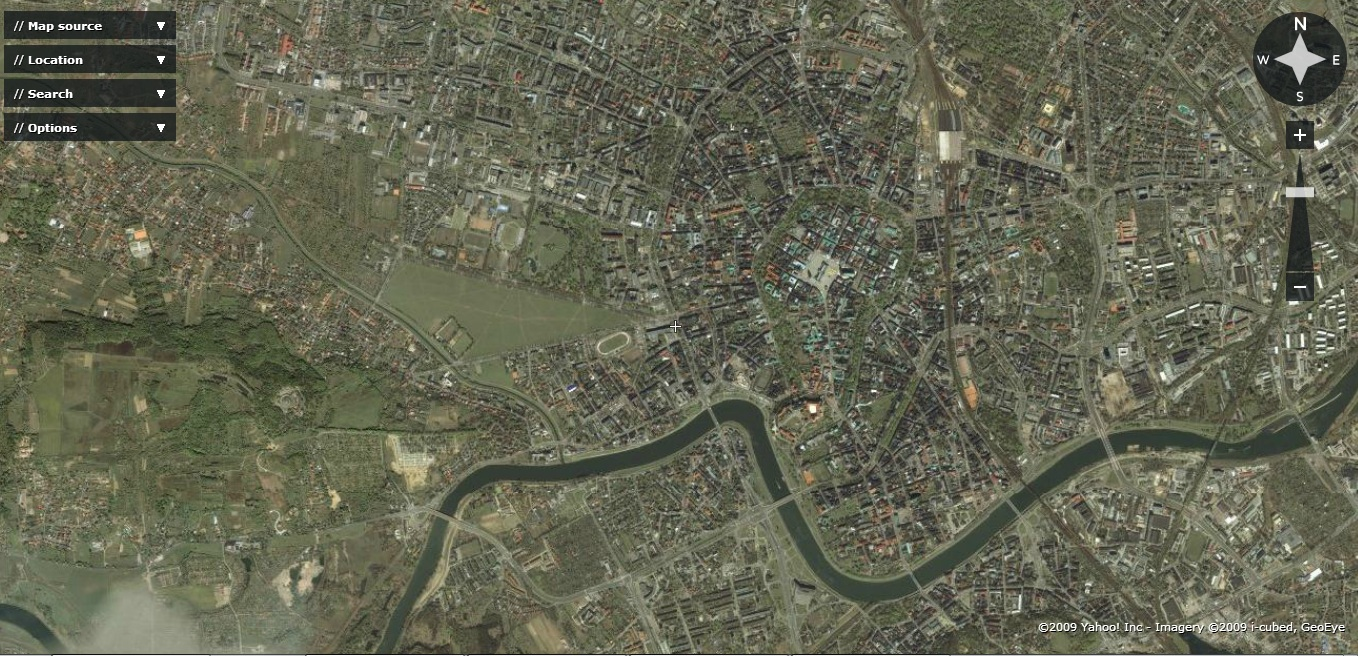
\includegraphics[width=100mm]{ge/yahoo_1.jpg}
  \caption{Yahoo Maps.}
  \label{fig:yahooMaps_1}
\end{figure}


\subsubsection{Apple Maps}
\label{subsec:Apple Maps}

Kolejną dużą marką która dostarcza informację jest Apple. Niestety nie ma wersji która pozwalałaby na dostęp do tej usługi z powszechnie używanych komputerów stacjonarnych. Dodatkowo jakość dostarczanych informacji jest bardzo złej jakości.


\subsection{SVG}
\label{subsec:svg}

Wstępny etap pracy zakładał wykorzystanie formatu SVG(en. Scalable Vector Graphics) do prezentacji danych, tworzenia animacji płynnych zmian kształtów.

Ciekawy przykład został zaprezentowany na stronie \underline{\texttt{http://www.svg-maps.com/sample\_zipcode\_map}} na której mapa po prawej stronie została w całości wygenerowana i dodano możliwość interakcji. Widok tej strony zaprezentowano na rysunku \ref{fig:svgmap}

\begin{figure}[H]
  \centering
    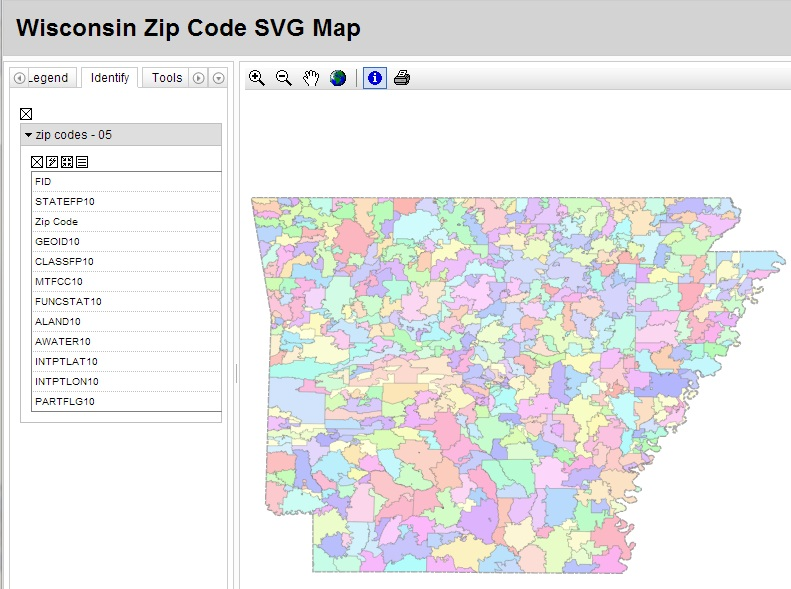
\includegraphics[width=120mm]{ge/svgmap.jpg}
  \caption{Wykorzystanie SVG}
  \label{fig:svgmap}
\end{figure}


\subsection{Canvas}
\label{sec:canvas}


Bardzo ciekawym i wartym zainteresowania dodanym elementem w nowej wersji jest obecność znaczniku canvas. Pozwala on na dynamiczne , skryptowe renderowanie kształtów i obrazów. Dzięki temu obiektowi możliwe stało się tworzenie animacji czy nawet gier działających w przeglądarce bez konieczności używania dodatkowych wtyczek czy programów.

\underline{\texttt{http://techtrendy.pl/title,Pierwsza-gra-3D-napisana-w-HTML5,wid,14102779,wiadomosc.html?ticaid=6107dc}}

Przykładem wielkich możliwości jakie dostarcza udoskonalony język jest fakt iż już w roku 2011 powstała pierwsza trójwymiarowa gra stworzona w całości przy użyciu HTML5. Przykład grafiki widoczny jest na rysunku \ref{fig:html3d}.
Wcześniej takie efekty możliwe były jednynie przy wykorzystaniu technologi Flash, jej wadą była drudność edycji gotowego produktu, wymagało to specjalnego oprogramowania. Fakt tworzenia pliku wykonywalnego którego nie było możliwości edycji wymuszał dostęp do kodów źródłowych, czyli plików które tworzył autor programu.

\begin{figure}[H]
  \centering
    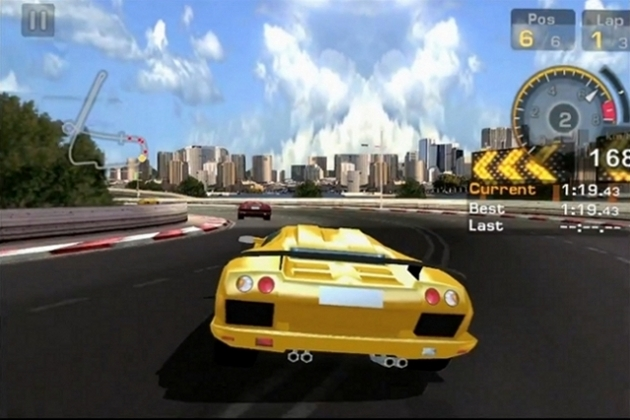
\includegraphics[width=100mm]{ge/html5_3d.jpg}
  \caption{Pierwsza gra 3D w html5.}
  \label{fig:html3d}
\end{figure}

Kolejną funkcjonalnością która wydaje się być przydatna w stosunku do omawianego projektu jest możliwość rysowania kształtów geomeycznych, również na innych obrazach. Przykładem wykorzystania tej technologi jest \ref{fig:canvas1} na którym przy pomocy okręgu zaznaczono rynek główny w Krakowie i jego okolice, możliwość zmiany przejżystości narysowanego kształtu pozwala aby obraz podnim był nadal widoczny.

  \begin{figure}[H]
  \centering
    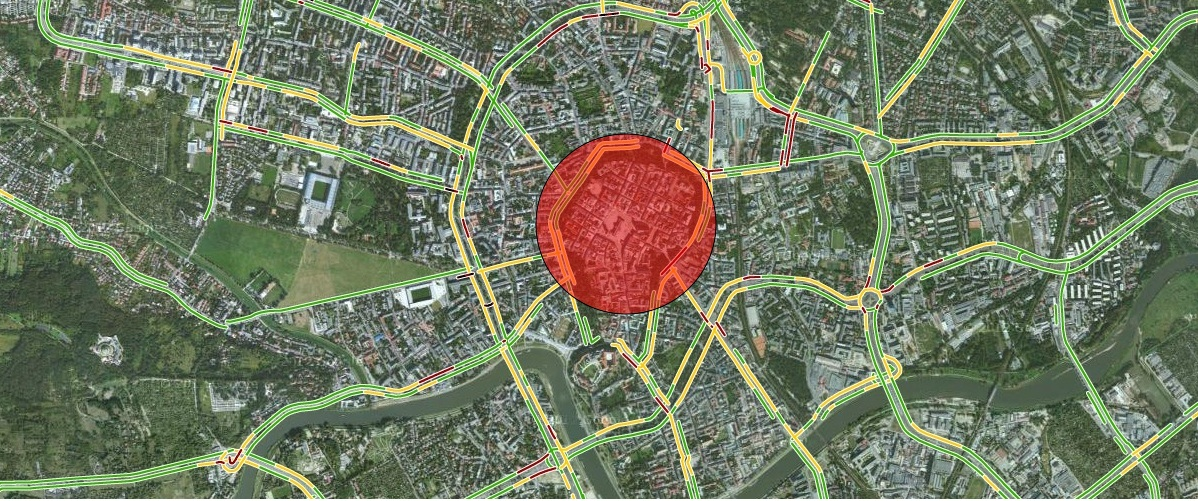
\includegraphics[width=100mm]{ge/canvas1.jpg}
  \caption{P.}
  \label{fig:canvas1}
\end{figure}

\lstset{language=JavaScript}
\begin{lstlisting}[caption=json]

      var canvas = document.getElementById('myCanvas');
      var context = canvas.getContext('2d');
      var imageObj = new Image();
	
      imageObj.onload = function() {
      context.drawImage(imageObj, 69, 50);
	  context.beginPath();
      context.arc(canvas.width / 2, canvas.height / 2, 90, 0, 2 * Math.PI, false);
      context.fillStyle = "rgba(255, 0, 0, 0.5)";
      context.fill();
      context.stroke();
      };
      imageObj.src = './gm_1.jpg';

\end{lstlisting}

\subsection{Google manager}
\label{sec:svg}

\subsection{Canvas2}
\label{sec:canvas2}
